\documentclass[12pt,letterpaper,onecolumn,openany,oneside]{book}
% Use draft option to be overfull 
\pdfoptionpdfminorversion 6
% Slightly newer pdf format outputted.  Helps compatability with included pdf images

%%%%%%%%%%%%%%%%%%%%%%%%%%%%
%%   additional packages  %%
%%%%%%%%%%%%%%%%%%%%%%%%%%%%
\usepackage{graphics,graphicx}         		% Figures
\usepackage{amsmath,amssymb,mathrsfs,bm} 	% Math symbols
\usepackage{tikz}                      		% Fancy drawings
% Extra packages mostly for flowchart--extra arrows, node positioning, diamond shape, aspect, vector add
\usetikzlibrary{arrows,positioning,shapes,shapes.geometric,calc}	
\usepackage{apalike}						% APA like bibliography style

%%%%%%%%%%%%%%%%%%%%%%%%%%%%
%%    Custom Commands     %%
%%%%%%%%%%%%%%%%%%%%%%%%%%%%
\newcommand{\angstrom}{\textup{\AA}}		% Angstrom command

%%%%%%%%%%%%%%%%%%%%%%%%%%%%
%%     Format             %%
%%%%%%%%%%%%%%%%%%%%%%%%%%%%
% Sets the margins--one sided document only odd commands are taken into effect
\usepackage[top=1.5in, bottom=1in, left=1.5in, right=1in]{geometry}
\setlength{\footskip}{.25in}				% Page numbers in footer are positioned bottom margin-\footskip from bottom of page to give 0.75"
\setlength{\headheight}{15pt}				% To avoid an error in fanyhdr
% Note: headers is automatically 1" from top of page like it should be
\usepackage{fancyhdr}						% Custom setup of header and footers which allows number positions to be placed
\usepackage[doublespacing]{setspace}		% Sets double spacing for main textand provides single spacing environment
\usepackage[font=doublespacing]{caption}	% Captions now also double spaced
\usepackage{sectsty}                  		% needed for the \allsectionsfont command
\allsectionsfont{\normalsize}				% Sets all section headers to 12 pt
\usepackage{layout}							% If you use the \layout command in the body of the text the formatting will be shown nicely

% Formatting still to do:
% No journal abbreviations in the bibliography (will have to manually edit :( )

\begin{document}
\mainmatter

\begin{figure}
	\begin{center}
	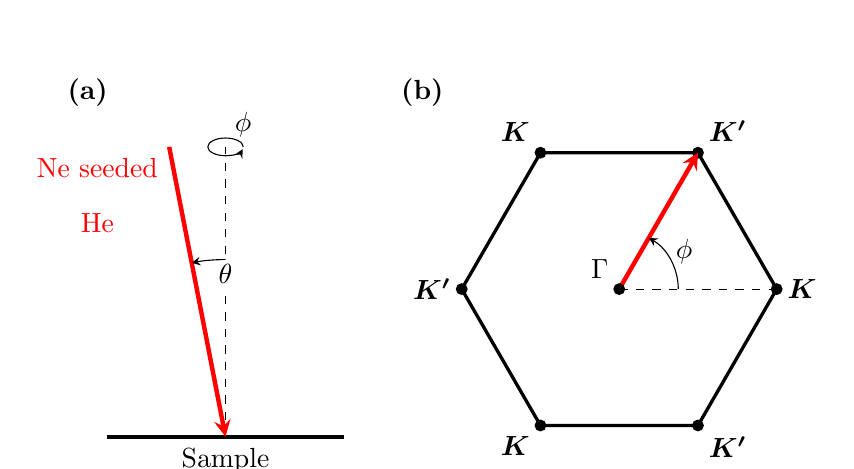
\begin{tikzpicture}
	% The experimental geometry
	\begin{scope}[ultra thick,>=stealth,scale=1.5,xshift=-2cm,yshift=-1.25cm]
		% The sample
		\draw (-1 cm, 0) -- node[below]{Sample} (1 cm, 0);
		% Normal line
		\draw[dashed,thin] (0,0) -- (0,0 |- 101:2.5 cm);
		% Incident Helium
		\draw[red,->] (90+11:2.5 cm) node[anchor=north east, align=center] {Ne seeded \\ He} -- (0:0);
		% Angle \theta
		\draw[thin,->] (0,1.5) 
			node[anchor=north, fill=white, opacity=1, text opacity=1,rounded corners=6 pt,inner sep=1.5 pt] {$\theta$} 
			arc(90:101:1.5 cm);
		% Angle \phi
		\draw[thin,->] (0.15,0 |- 101:2.5 cm) 
			node[anchor=south] {$\phi$} 
			arc(0:345:.15 cm and .075 cm);
	\end{scope}

	% Reciprocal space with red arrow indicating the direction of the excited phonon
	\begin{scope}[xshift=2cm,
		BZ/.style={color=black,fill=black,very thick},
		circ2/.style={radius=1.5pt}]

		% Draw the BZ
		\draw[BZ]
			(  0:2 cm) circle[circ2] node[anchor=west      ]{$\bm{K} $} --
			( 60:2 cm) circle[circ2] node[anchor=south west]{$\bm{K'}$} --
			(120:2 cm) circle[circ2] node[anchor=south east]{$\bm{K }$} -- 
			(180:2 cm) circle[circ2] node[anchor=east      ]{$\bm{K'}$} -- 
			(240:2 cm) circle[circ2] node[anchor=north east]{$\bm{K }$} -- 
			(300:2 cm) circle[circ2] node[anchor=north west]{$\bm{K'}$} -- 
			(  0:2 cm);

		% The excited phonon
		\draw[ultra thick,red,>=stealth,->] (0,0) -- (60:2 cm);
		% The angle
		\draw[thin,dashed,black] (0,0) -- (2 cm,0);
		\draw[thin,>=stealth,->,black] (.75 cm,0) arc(0:60:.75 cm);
		\node at (30:.95) {$\phi$};

		% Label the high symmetry points
		\draw[BZ] (0,0) circle[circ2] node[anchor=south east]{$\Gamma$};
	\end{scope}

	% Figure labels
	\node at (-4.75cm, 2.5 cm) {\textbf{(a)}};
	\node at (-.5cm, 2.5 cm) {\textbf{(b)}};
\end{tikzpicture}
	\end{center}
\end{figure}

\end{document}